\chapter{Experiments}
\label{chap:experiments}

In this chapter, the experiments and results of this work are displayed. First, we establish the general experimental setup. Afterwards, the results of the conducted MVTecAD LOCO \cite{LOCODentsAndScratchesBergmann2022}
survey are presented in section \ref{sec:locoxperiments}. As a baseline for performance evaluation, we utilize the performance on the more conventional MVTecAD dataset \cite{MVTEC_Bergmann_2021} and a classifier comparison. In section \ref{sec:faltconnectorxperiments}, we review the performance of the classifiers on our novel dataset category. Lastly section \ref{sec:ensembleresults} 
deals with the ensemble network approach findings, which were also conducted on the MVTecAD LOCO dataset and the new dataset category introduced in this work.


\section{Experimental Setup}
\label{sec:experimentsetup}

All model training and result reproductions have been conducted on the IAD cluster student partition. The GPU in use for all nodes used by that partition is an 
RTX 2080Ti with 11GB of memory, and the CPU is an AMD Ryzen 9 16-Core processor. The cluster overview \cite{clusterdocs} serves to provide further detail for additional questions. 
As for software, the specifications of other libraries, as well as the specifications for the MVTecAD LOCO experiment, are documented in the 
environment files in the project code.



\section{MVTecAD LOCO Experiments}
\label{sec:locoxperiments}

In this section, we review the performance of the IAD methods mentioned in section \ref{sec:IADmethods} on the MVTecAD LOCO \cite{LOCODentsAndScratchesBergmann2022} 
dataset. Tables \ref{tab:imageaurocloco}, \ref{tab:pixelaurocloco}, and \ref{tab:sproloco} each display the experiments with regards to one of the metrics: image AUROC, pixel AUROC and sPRO. \newline
Comparing the average image and pixel AUROCs to the ones reported in the chapter \ref{chap:background}, a decrease in performance is visible. 
This is also true regarding the average pixel-wise AUROC. The performances of the classifiers were on a similar level, emphasizing that all these approaches can achieve equally high-quality results. Reverse Destillation \cite{revdist2023} displayed a slightly more significant performance drop in pixel AUROC, while PatchCore \cite{patchCore2022} 
did barely lose in that category.

\begin{table}[htbp]
    \tiny
    \centering
    \begin{tabularx}{\textwidth}{|X|X|X|X|X|X|X|}%{|c|p{5cm}|p{5cm}|p{5cm}|}
        \hline
        \textbf{Method} & \textbf{Breakfast Box} & \textbf{Juice Bottle} & \textbf{Pushpins} & \textbf{Scew Bag} & \textbf{Splicing Connectors} & \textbf{Average} \\
        \hline
        PC \cite{patchCore2022} & 1.0 & 0.997 & 0.981 & 0.982 & 0.983 & 1.0 \\
        \hline
        SN \cite{liu2023simplenet} & 0.887 & 0.878 & 0.765 & 0.768 & 0.725 & 0.803 \\
        \hline
        CS \cite{csflow2022} & 0.998 & 0.991 & 0.971 & 1.0 & 0.990 & 0.996 \\
        \hline
        DRAEM \cite{Zavrtanik_2021DRAEM} & 0.992 & 0.918 & 0.985 & 0.970 & 0.999 & 1.0 \\
        \hline
        RevDist \cite{revdist2023} & 1.0 & 0.992 & 0.990 & 1.0 & 1.0 & 1.0 \\
        \hline
    \end{tabularx}
    \caption{Collection of image auroc results of reviewed IAD methods on the MVTecAD LOCO \cite{LOCODentsAndScratchesBergmann2022} dataset.}
    \label{tab:imageaurocloco}
\end{table}

When investigating column-wise performance, we found that the dataset classes seem to have varying challenge levels. Albeit some fluctuations, 
the juice bottle class consistently gets very high results in image and pixel AUROC, especially regarding the latter. 
Conversely, the class screw bag seems to have lower image AUROC results often.

\begin{table}[htbp]
    \tiny
    \centering
    \begin{tabularx}{\textwidth}{|X|X|X|X|X|X|X|}%{|c|p{5cm}|p{5cm}|p{5cm}|}
        \hline
        \textbf{Method} & \textbf{Breakfast Box} & \textbf{Juice Bottle} & \textbf{Pushpins} & \textbf{Screw Bag} & \textbf{Splicing Connectors} & \textbf{Average} \\
        \hline
        PC \cite{patchCore2022} & 0.864 & 0.991 & 0.961 & 0.920 & 0.867 & 0.920 \\
        \hline 
        SN \cite{liu2023simplenet} & 0.652 & 0.962 & 0.926 & 0.794 & 0.079 & 0.682 \\
        \hline %----- up side done ------
        CS \cite{csflow2022} & 0.998 & 0.991 & 0.971 & 1.0 & 0.990 & 0.996 \\
        \hline
        DRAEM \cite{Zavrtanik_2021DRAEM} & 0.992 & 0.918 & 0.985 & 0.970 & 0.999 & 1.0 \\
        \hline
        RevDist \cite{revdist2023} & 1.0 & 0.992 & 0.990 & 1.0 & 1.0 & 1.0 \\
        \hline
    \end{tabularx}
    \caption{Collection of pixel auroc results of reviewed IAD methods on the MVTecAD LOCO \cite{LOCODentsAndScratchesBergmann2022} dataset.}
    \label{tab:pixelaurocloco}
\end{table}








The sPRO values calculated for the approaches were of below-average performance, as seen in table \ref{tab:sproloco}. Despite this, the results seem legitimate when comparing the metrics to the 
class averages reported in \cite{LOCODentsAndScratchesBergmann2022}. Bergmann et al. review methods 
in this paper that they selected to be applicable to logical anomalies. The classifiers in this survey cannot compete with their novel IAD method GCAD, which reaches an 
average sPRO of 0.701. Still, they were sometimes in comparable regions as other classifiers in the named paper, producing an expected performance. 
The average metric scores are all very close to each other, suggesting equal performance in the end.


\begin{table}[htbp]
    \tiny
    \centering
    \begin{tabularx}{\textwidth}{|X|X|X|X|X|X|X|}%{|c|p{5cm}|p{5cm}|p{5cm}|}
        \hline
        \textbf{Method} & \textbf{Breakfast Box} & \textbf{Juice Bottle} & \textbf{Pushpins} & \textbf{Screw Bag} & \textbf{Splicing Connectors} & \textbf{Average} \\
        \hline
        PC \cite{patchCore2022} & 0.124 & 0.244 & 0.406 & 0.373 & 0.212 & 0.272 \\
        \hline 
        SN \cite{liu2023simplenet} & 0.108 & 0.229 & 0.395 & 0.360 & 0.197 & 0. \\
        \hline
        DRAEM \cite{Zavrtanik_2021DRAEM} & 0. & 0. & 0. & 0. & 0. &  \\
        \hline
        RevDist \cite{revdist2023} & .0 & 0. & 0. & .0 & .0 & .0 \\
        \hline
    \end{tabularx}
    \caption{Collection of pixel auroc results of reviewed IAD methods on the MVTecAD LOCO \cite{LOCODentsAndScratchesBergmann2022} dataset.}
    \label{tab:sproloco}
\end{table}





To bring the numbers mentioned above into perspective, the drop of an image and pixel level AUROC for the classifiers between the 
MVTecAD \cite{MVTEC_Bergmann_2021} and the MVTecAD LOCO \cite{LOCODentsAndScratchesBergmann2022} dataset was significant. Approaches 
PatchCore \cite{patchCore2022}, SimpleNet \cite{liu2023simplenet}, Reverse Distillation \cite{revdist2023} and DRAEM \cite{Zavrtanik_2021DRAEM} had a fall off 
in image AUROC class average of respectively 0.174, 0.193, 0.208 and 0.213. Concerning the pixel-wise 
AUROC, a decline of 0.064, 0.147, 0.218 and 0.174 emerged. \newline
Fig. \ref{fig:structvslogic} shows exemplary metrics divided by structural and logical anomalies. The reported pixel AUROCs slightly differ from earlier reported results due to a different 
evaluation split of good images, but they showcase a principal performance difference. Here, better performance is visible for the 
class of structural anomalies, sometimes even by up to 29 percent, suggesting that logical anomalies are distinctively more challenging to segment correctly.

\begin{figure}[H]
    \centering
    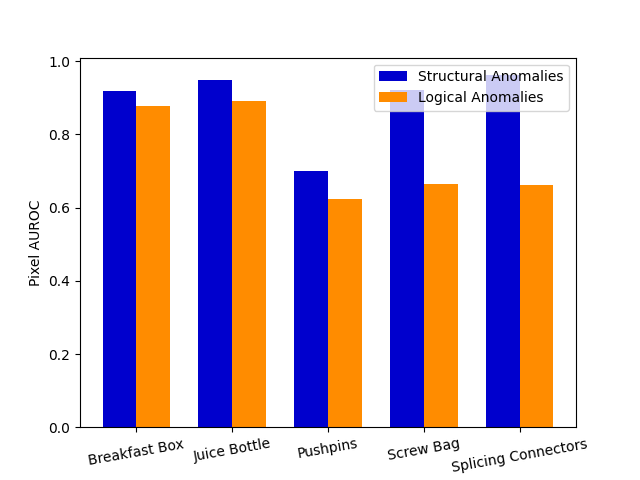
\includegraphics[width=0.5\textwidth]{figures/structvslogic.png}
    \caption{Exemplary pixel AUROC comparison of PatchCore \cite{patchCore2022} between structural and logical anomalies. For each evaluation class, all normal class images 
             are taken into calculation, resulting in deviating AUROCS from the original reported ones.}
    \label{fig:structvslogic}
\end{figure}

Additionally, below in Fig. \ref{fig:locoallapproaches} are representative images from multiple classes that showcase good and bad segmentation results. Results are taken from multiple approaches, and more results can be found in the appendix. The following subsection deals with the strengths and weaknesses of individual classifiers found when examining the images.

%\begin{figure}[htbp]
    \captionsetup[subfigure]{justification=centering}
    \centering
    \begin{subfigure}[b]{0.3\textwidth}
        \centering
        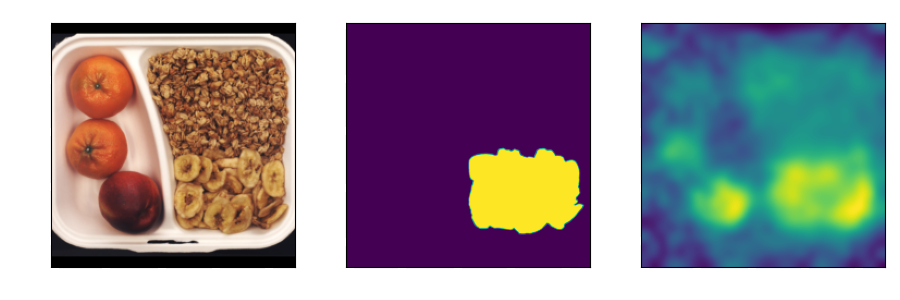
\includegraphics[width=\textwidth]{figures/locopatchcoreresults/breakfast_box_test_logical_anomalies_003.png}
        %\caption*{Logical Anomalies}

    \end{subfigure}
    \begin{subfigure}[b]{0.3\textwidth}
        \centering
        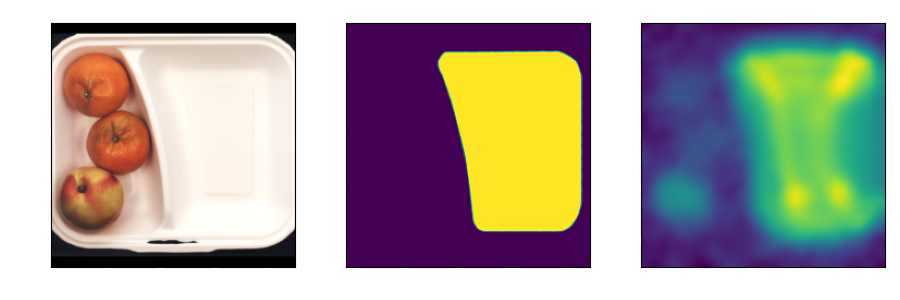
\includegraphics[width=\textwidth]{figures/locopatchcoreresults/breakfast_box_test_logical_anomalies_034.png}


    \end{subfigure}
    \begin{subfigure}[b]{0.3\textwidth}
        \centering
        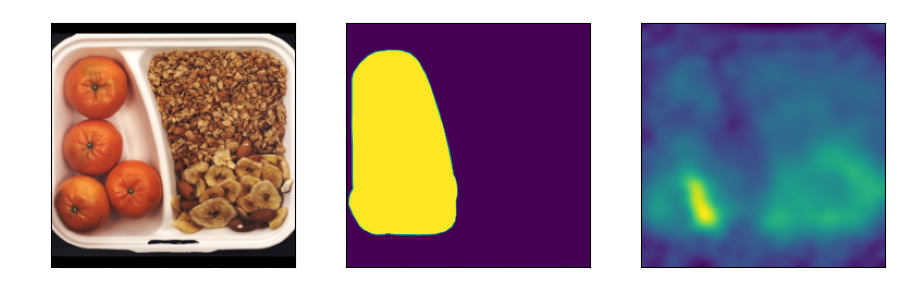
\includegraphics[width=\textwidth]{figures/locopatchcoreresults/breakfast_box_test_logical_anomalies_070.png}


    \end{subfigure}
    \begin{subfigure}[b]{0.3\textwidth}
        \centering
        \includegraphics[width=\textwidth]{figures/locopatchcoreresults/breakfast_box_test_structural_anomalies_014.png}
        %\caption*{Structural Anomalies}

    \end{subfigure}
    \begin{subfigure}[b]{0.3\textwidth}
        \centering
        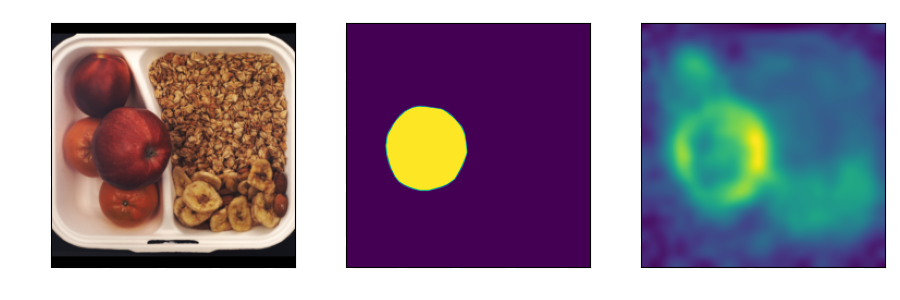
\includegraphics[width=\textwidth]{figures/locopatchcoreresults/breakfast_box_test_structural_anomalies_024.png}


    \end{subfigure}
    \begin{subfigure}[b]{0.3\textwidth}
        \centering
        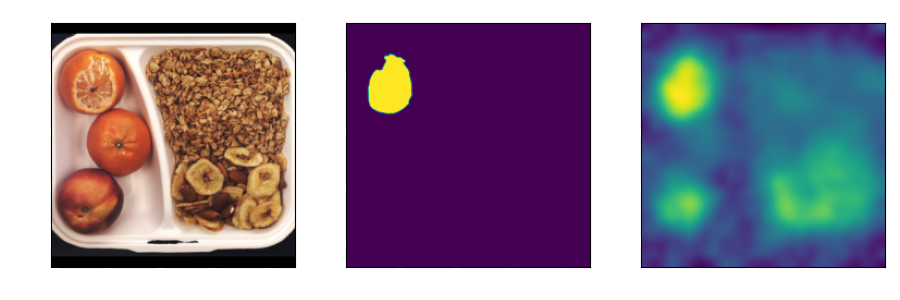
\includegraphics[width=\textwidth]{figures/locopatchcoreresults/breakfast_box_test_structural_anomalies_070.png}


    \end{subfigure}
    \caption{Exemplary Results of PatchCore on the Breakfast Box Class}
    \label{fig:PCBB}
\end{figure}
%\begin{figure}[htbp]
    \captionsetup[subfigure]{justification=centering}
    \centering
    \begin{subfigure}[b]{0.3\textwidth}
        \centering
        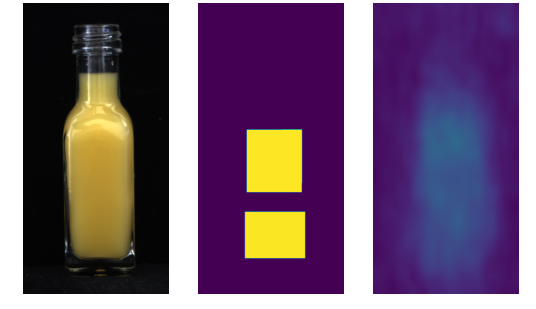
\includegraphics[width=\textwidth]{figures/locosimplenetresults/JB/image_prediction_105.png}
        %\caption*{Logical Anomalies}

    \end{subfigure}
    \begin{subfigure}[b]{0.3\textwidth}
        \centering
        \includegraphics[width=\textwidth]{figures/locosimplenetresults/JB/image_prediction_188.png}

    \end{subfigure}
    \begin{subfigure}[b]{0.3\textwidth}
        \centering
        \includegraphics[width=\textwidth]{figures/locosimplenetresults/JB/image_prediction_258.png}

    \end{subfigure}
    \begin{subfigure}[b]{0.3\textwidth}
        \centering
        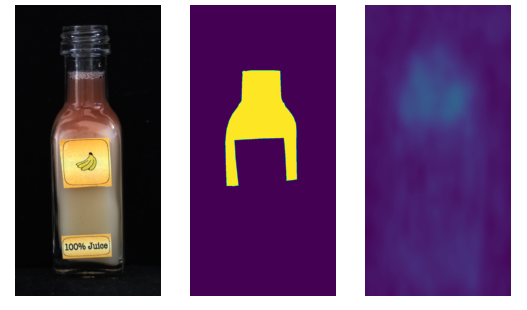
\includegraphics[width=\textwidth]{figures/locosimplenetresults/JB/image_prediction_286.png}
                %\caption*{Structural Anomalies}

    \end{subfigure}
    \begin{subfigure}[b]{0.3\textwidth}
        \centering
        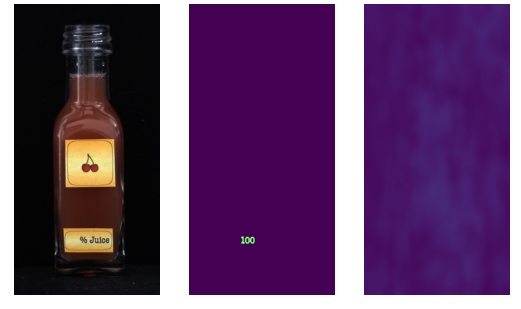
\includegraphics[width=\textwidth]{figures/locosimplenetresults/JB/image_prediction_297.png}

    \end{subfigure}
    \begin{subfigure}[b]{0.3\textwidth}
        \centering
        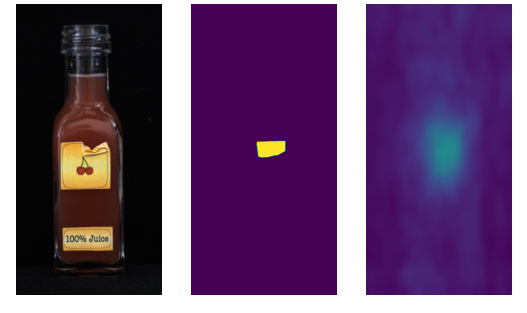
\includegraphics[width=\textwidth]{figures/locosimplenetresults/JB/image_prediction_300.png}

    \end{subfigure}
    \caption{Exemplary Results of SimpleNet on the Juice Bottle Class}
    \label{fig:SNJB}
\end{figure}

\begin{figure}[H]
    \captionsetup[subfigure]{justification=centering}
    \centering
    \begin{subfigure}[b]{\textwidth}
        \centering
        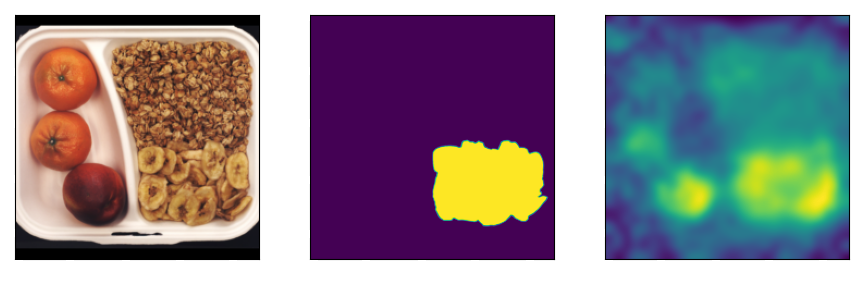
\includegraphics[width=0.45\textwidth]{figures/locoallapproaches/patchcore/breakfast_box_test_logical_anomalies_003.png}
        \includegraphics[width=0.45\textwidth]{figures/locoallapproaches/patchcore/breakfast_box_test_structural_anomalies_014.png}
        \caption{PatchCore \cite{patchCore2022} classifier results.}

    \end{subfigure}
    \begin{subfigure}[b]{\textwidth}
        \centering
        \includegraphics[width=0.45\textwidth]{figures/locoallapproaches/simplenet/image_prediction_188.png}
        \includegraphics[width=0.45\textwidth]{figures/locoallapproaches/simplenet/image_prediction_258.png}
        \caption{SimpleNet \cite{liu2023simplenet} classifier results.}

    \end{subfigure}
    \begin{subfigure}[b]{\textwidth}
        \centering
        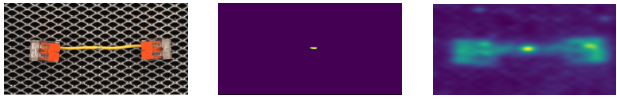
\includegraphics[width=0.45\textwidth]{figures/locoallapproaches/RevDist/revdist_003.png}
        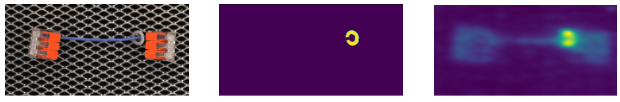
\includegraphics[width=0.45\textwidth]{figures/locoallapproaches/RevDist/RevDist_053.png}
        \caption{Reverse Distillation \cite{revdist2023} classifier results.}

    \end{subfigure}
    \begin{subfigure}[b]{\textwidth}
        \centering
        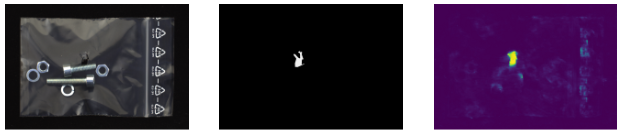
\includegraphics[width=0.45\textwidth]{figures/locoallapproaches/DRAEM/DRAEM_SB.png}
        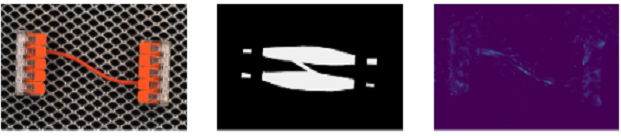
\includegraphics[width=0.45\textwidth]{figures/locoallapproaches/DRAEM/DRAEM_SC.png}
        \caption{DRAEM \cite{Zavrtanik_2021DRAEM} classifier results.}

    \end{subfigure}
    
    \caption{Representative segmentation results from all classifiers on the breakfast box class of the MVTecAD LOCO \cite{LOCODentsAndScratchesBergmann2022} dataset.}
    \label{fig:locoallapproaches}
\end{figure}


\subsection{Classifier Behavior}
\label{subsec:classifierbehavior}

Some classifiers exhibited different strengths and weaknesses when inspecting localization performance in segmented images. Fig. \ref{fig:sameimagecomparison} showcases 
the performance comparison between the classifiers on an arbitrary image from the dataset.

\begin{figure}[H]
    \captionsetup[subfigure]{justification=centering}
    \centering
    \begin{subfigure}[b]{0.45\textwidth}
        \centering
        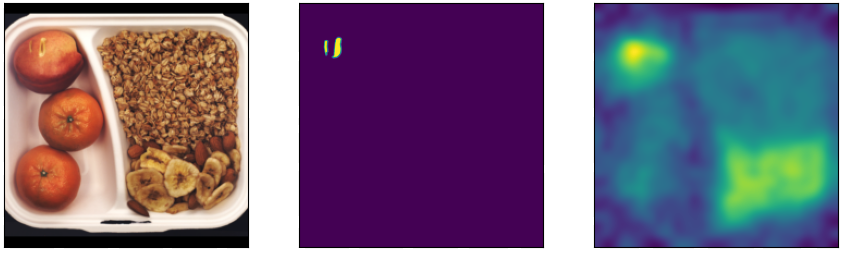
\includegraphics[width=\textwidth]{figures/sameimagecomparison/breakfast_box_test_structural_anomalies_059.png}
        \caption{PatchCore \cite{patchCore2022} classifier results.}

    \end{subfigure}
    \begin{subfigure}[b]{0.45\textwidth}
        \centering
        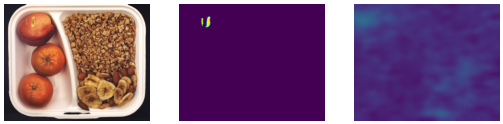
\includegraphics[width=\textwidth]{figures/sameimagecomparison/image_prediction_244.png}
        \caption{SimpleNet \cite{liu2023simplenet} classifier results.}

    \end{subfigure}
    \begin{subfigure}[b]{0.45\textwidth}
        \centering
        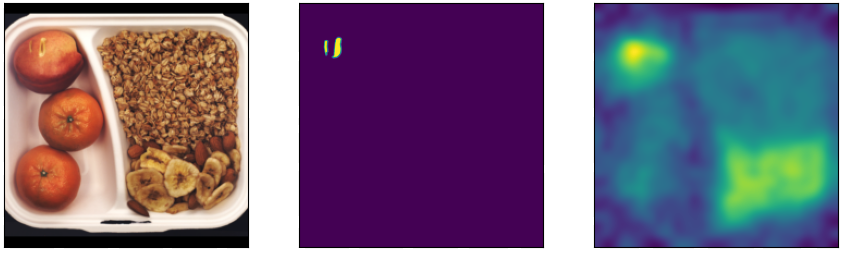
\includegraphics[width=\textwidth]{figures/sameimagecomparison/breakfast_box_test_structural_anomalies_059.png}
        \caption{Reverse Distillation \cite{revdist2023} classifier results.}

    \end{subfigure}
    \begin{subfigure}[b]{0.45\textwidth}
        \centering
        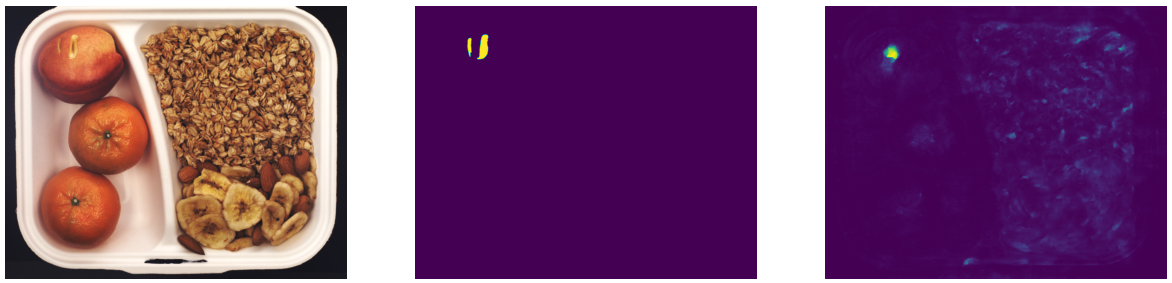
\includegraphics[width=\textwidth]{figures/sameimagecomparison/BB_DRAEM.png}
        \caption{DRAEM \cite{Zavrtanik_2021DRAEM} classifier results.}

    \end{subfigure}
    
    \caption{Comparison of classifier results on the same image.}
    \label{fig:sameimagecomparison}
\end{figure}

DRAEM \cite{Zavrtanik_2021DRAEM}, for instance, often showed exact localization performance in multiple classes but struggled 
with correctly segmenting anomalies in cases where objects are missing and there is no visible border on where this object should 
appear. For instance, precisely localizing missing nuts in the right compartment of the breakfast box class was done well, yet 
segmenting a missing screw that could be anywhere in the screw bag was often barely done at all (Fig. \ref{fig:DRAEMweakness}). As these logical anomalies occur 
frequently in the MVTecAD LOCO \cite{LOCODentsAndScratchesBergmann2022} dataset, it also explains how DRAEM 
has the most significant drop in average performance among the classifiers despite its mostly precise localization. Another aspect of this result is that DRAEM is very strict with 
segmentations. Often, results are perfectly interpretable by humans but may perform worse than other segmentations, as DRAEM does not necessarily segment all pixels in 
an anomalous region.

\begin{figure}[H]
    \centering
    \begin{subfigure}[b]{0.48\textwidth}
        \centering
        \begin{minipage}{0.32\textwidth}
            \centering
            \includegraphics[width=\textwidth]{figures/DRAEMweakness/structural026image.png}
        \end{minipage}
        \begin{minipage}{0.32\textwidth}
            \centering
            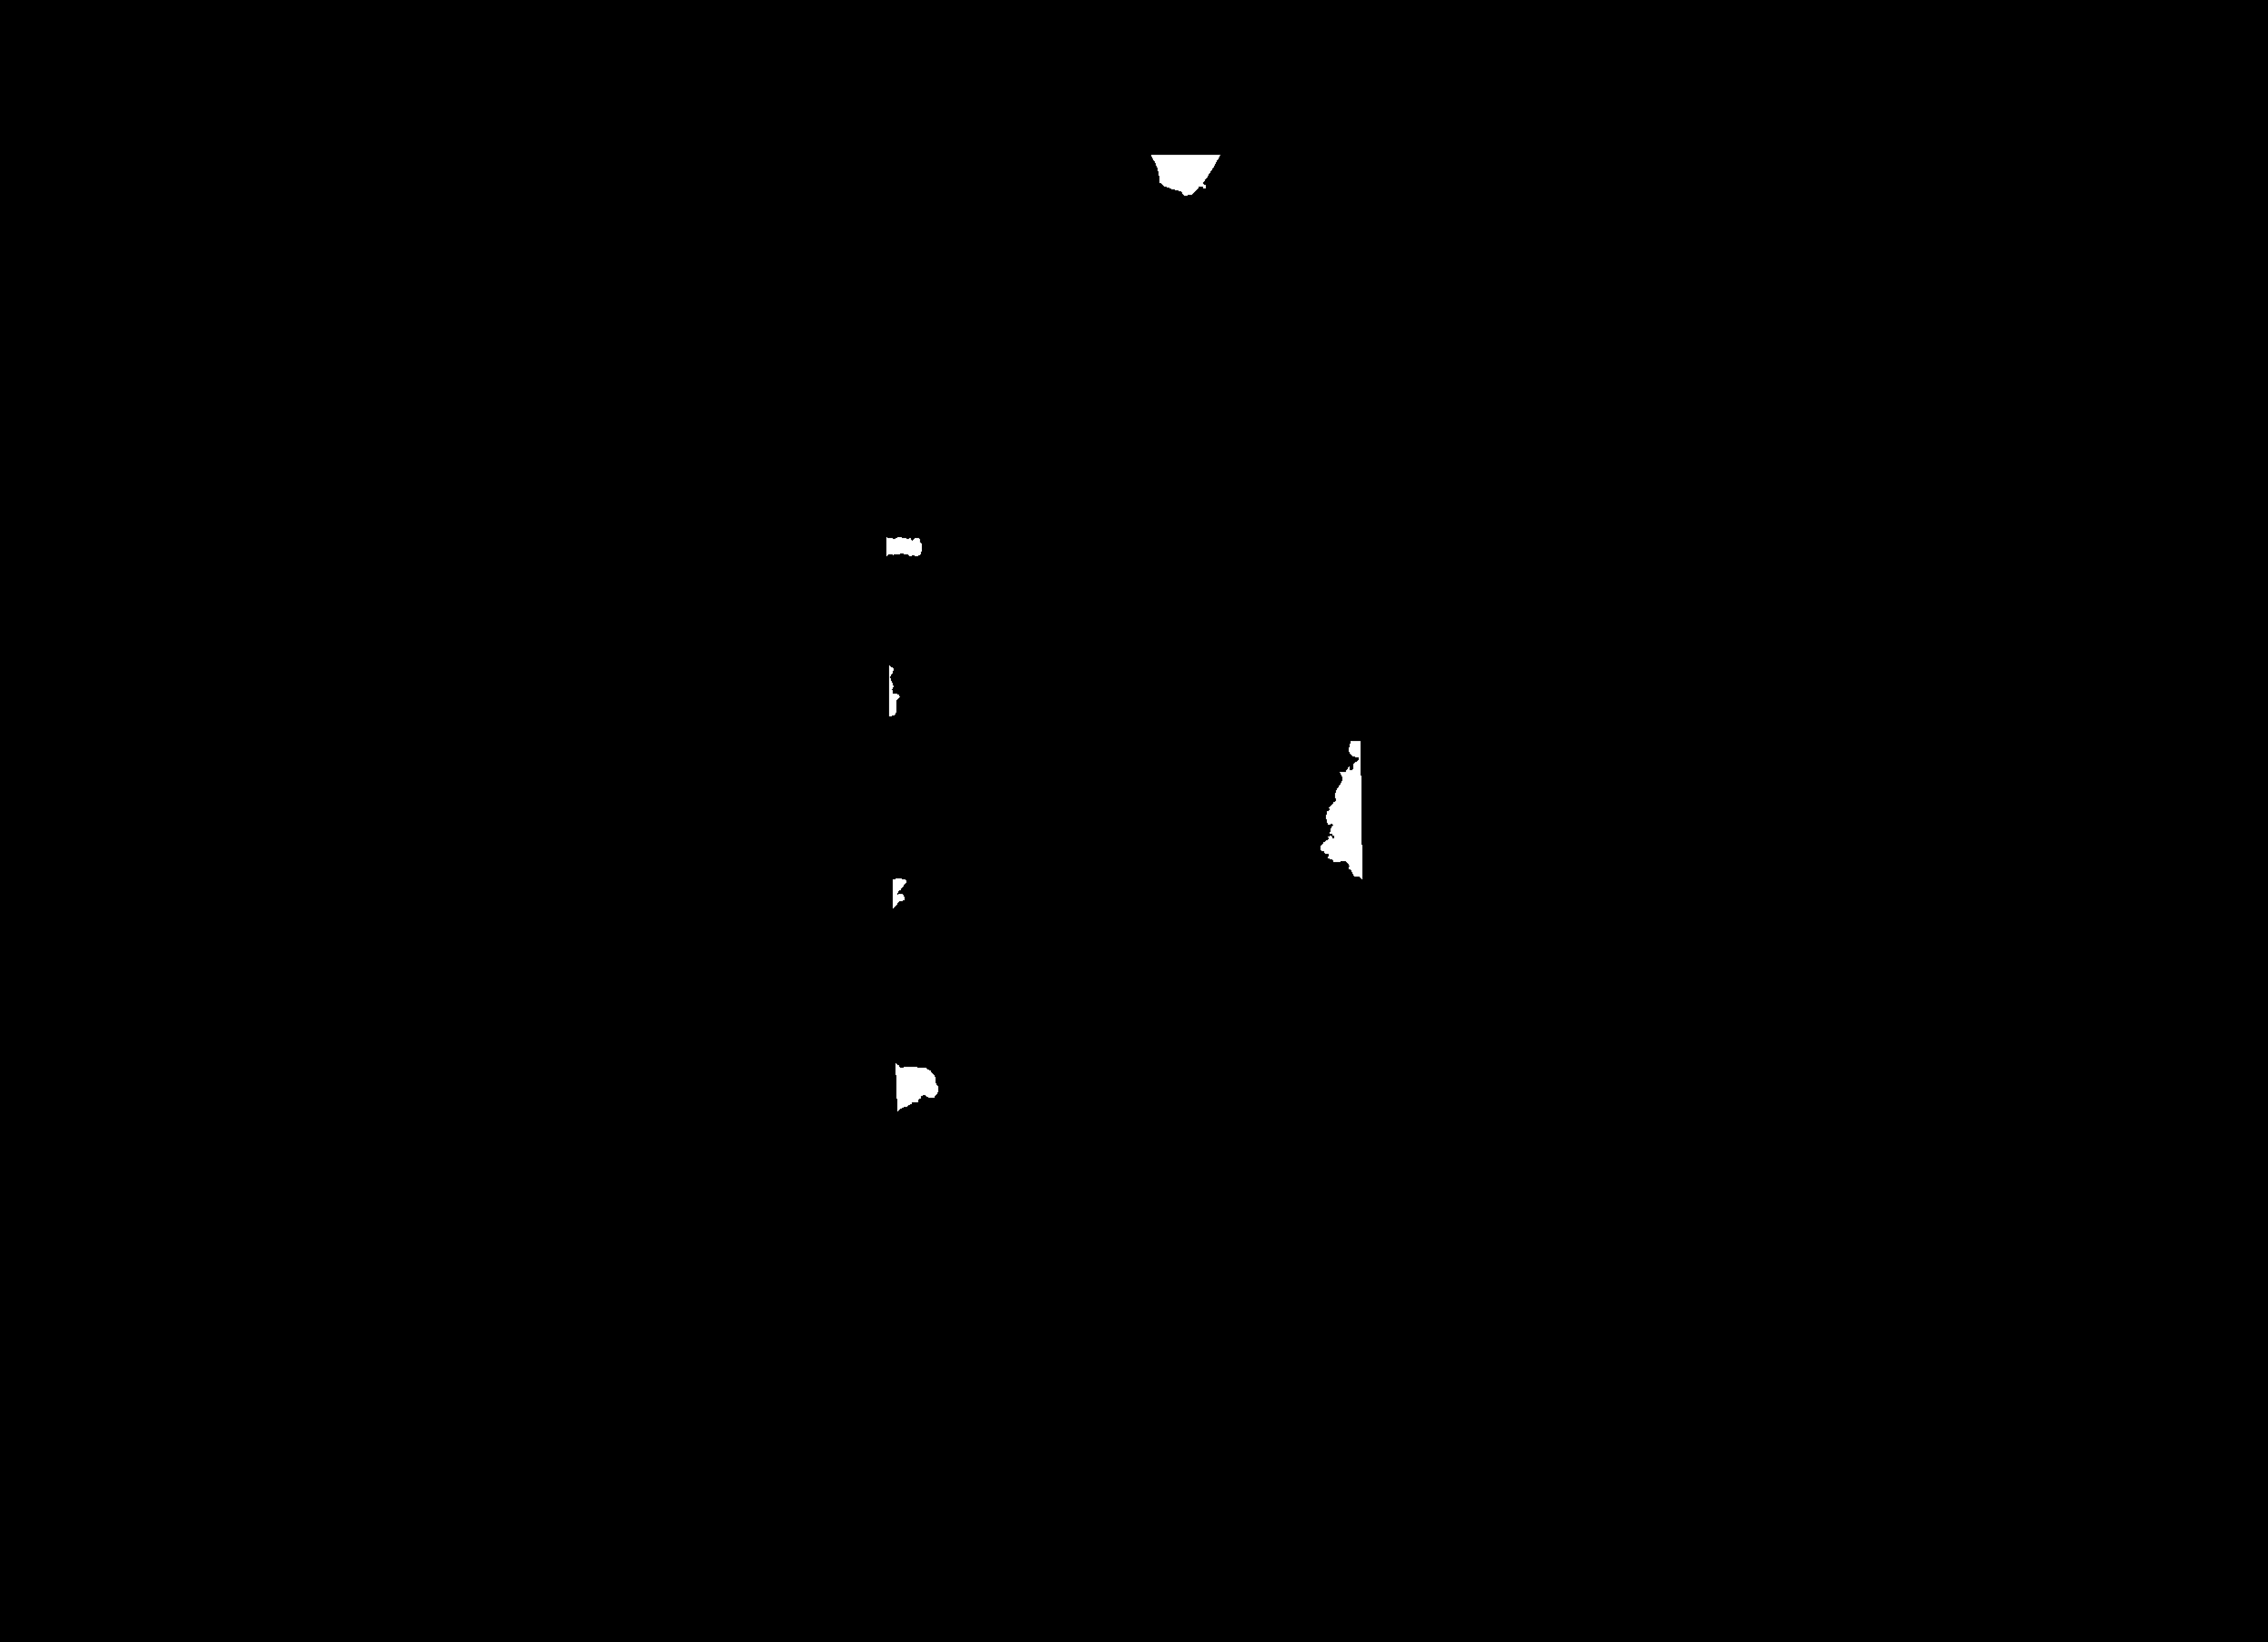
\includegraphics[width=\textwidth]{figures/DRAEMweakness/structural026mask.png}
        \end{minipage}
        \begin{minipage}{0.32\textwidth}
            \centering
            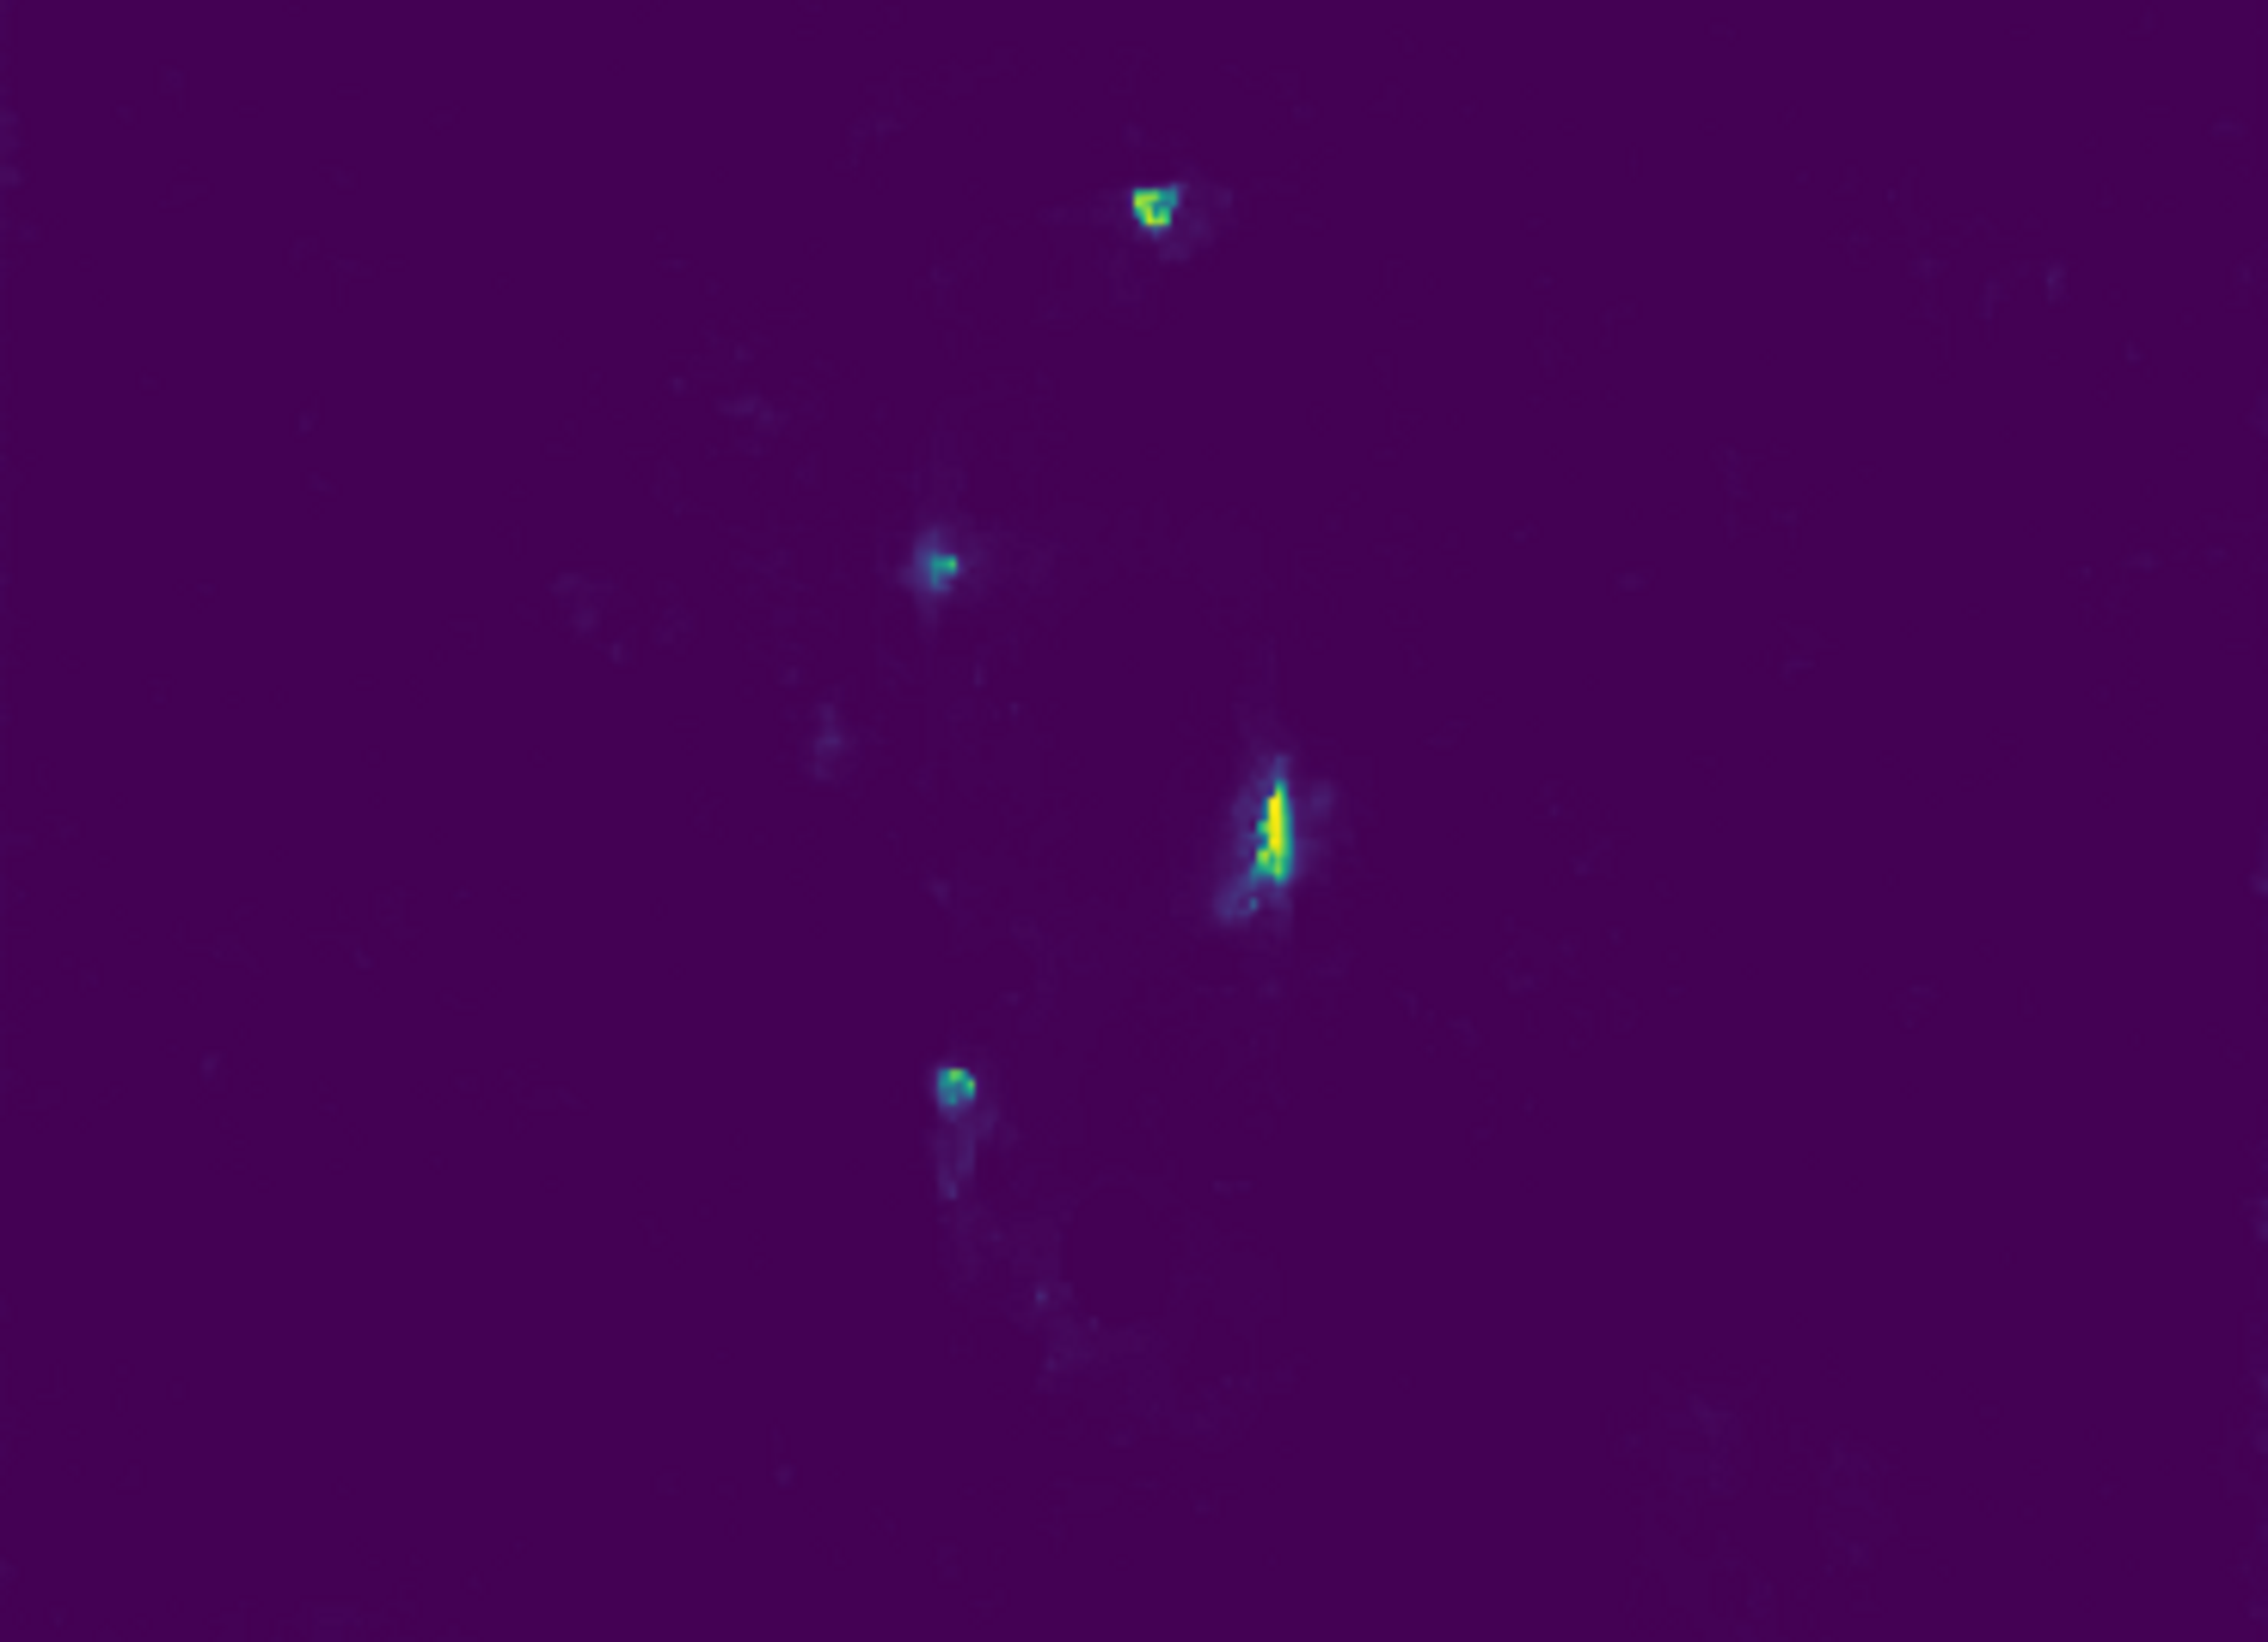
\includegraphics[width=\textwidth]{figures/DRAEMweakness/structural026segment.png}
        \end{minipage}
    \end{subfigure}
    \hfill
    \begin{subfigure}[b]{0.48\textwidth}
        \centering
        \begin{minipage}{0.32\textwidth}
            \centering
            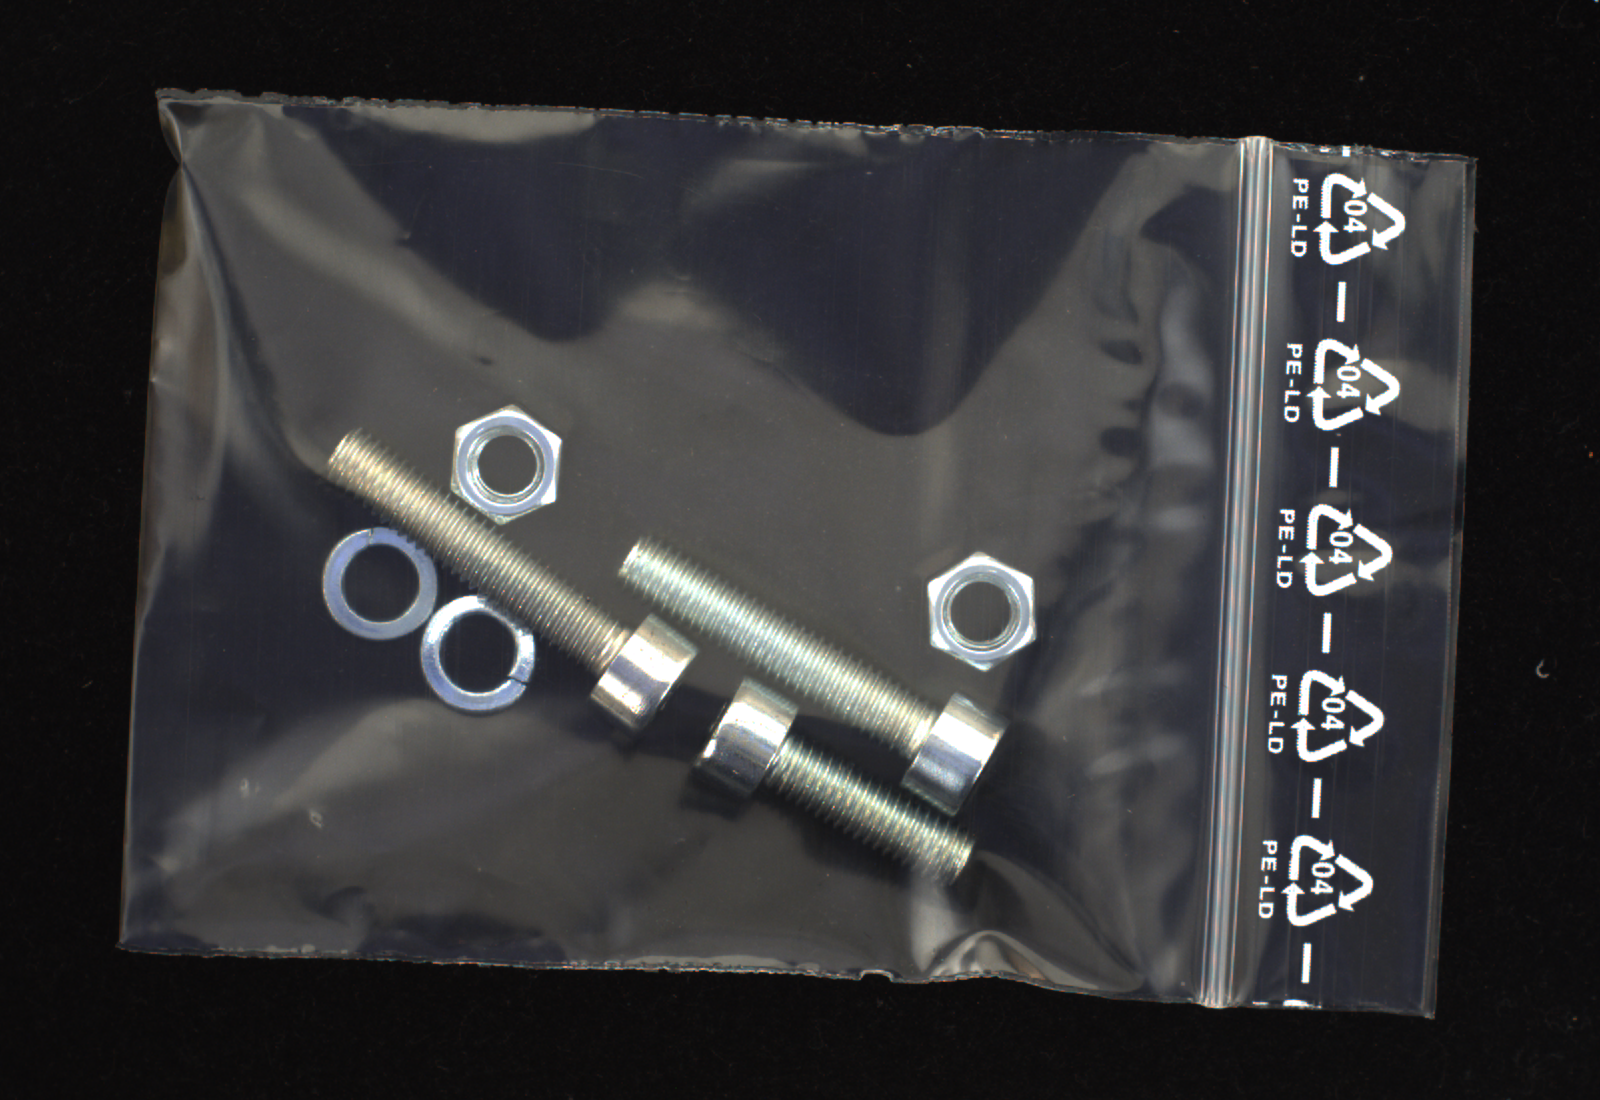
\includegraphics[width=\textwidth]{figures/DRAEMweakness/logical042image.png}
        \end{minipage}
        \begin{minipage}{0.32\textwidth}
            \centering
            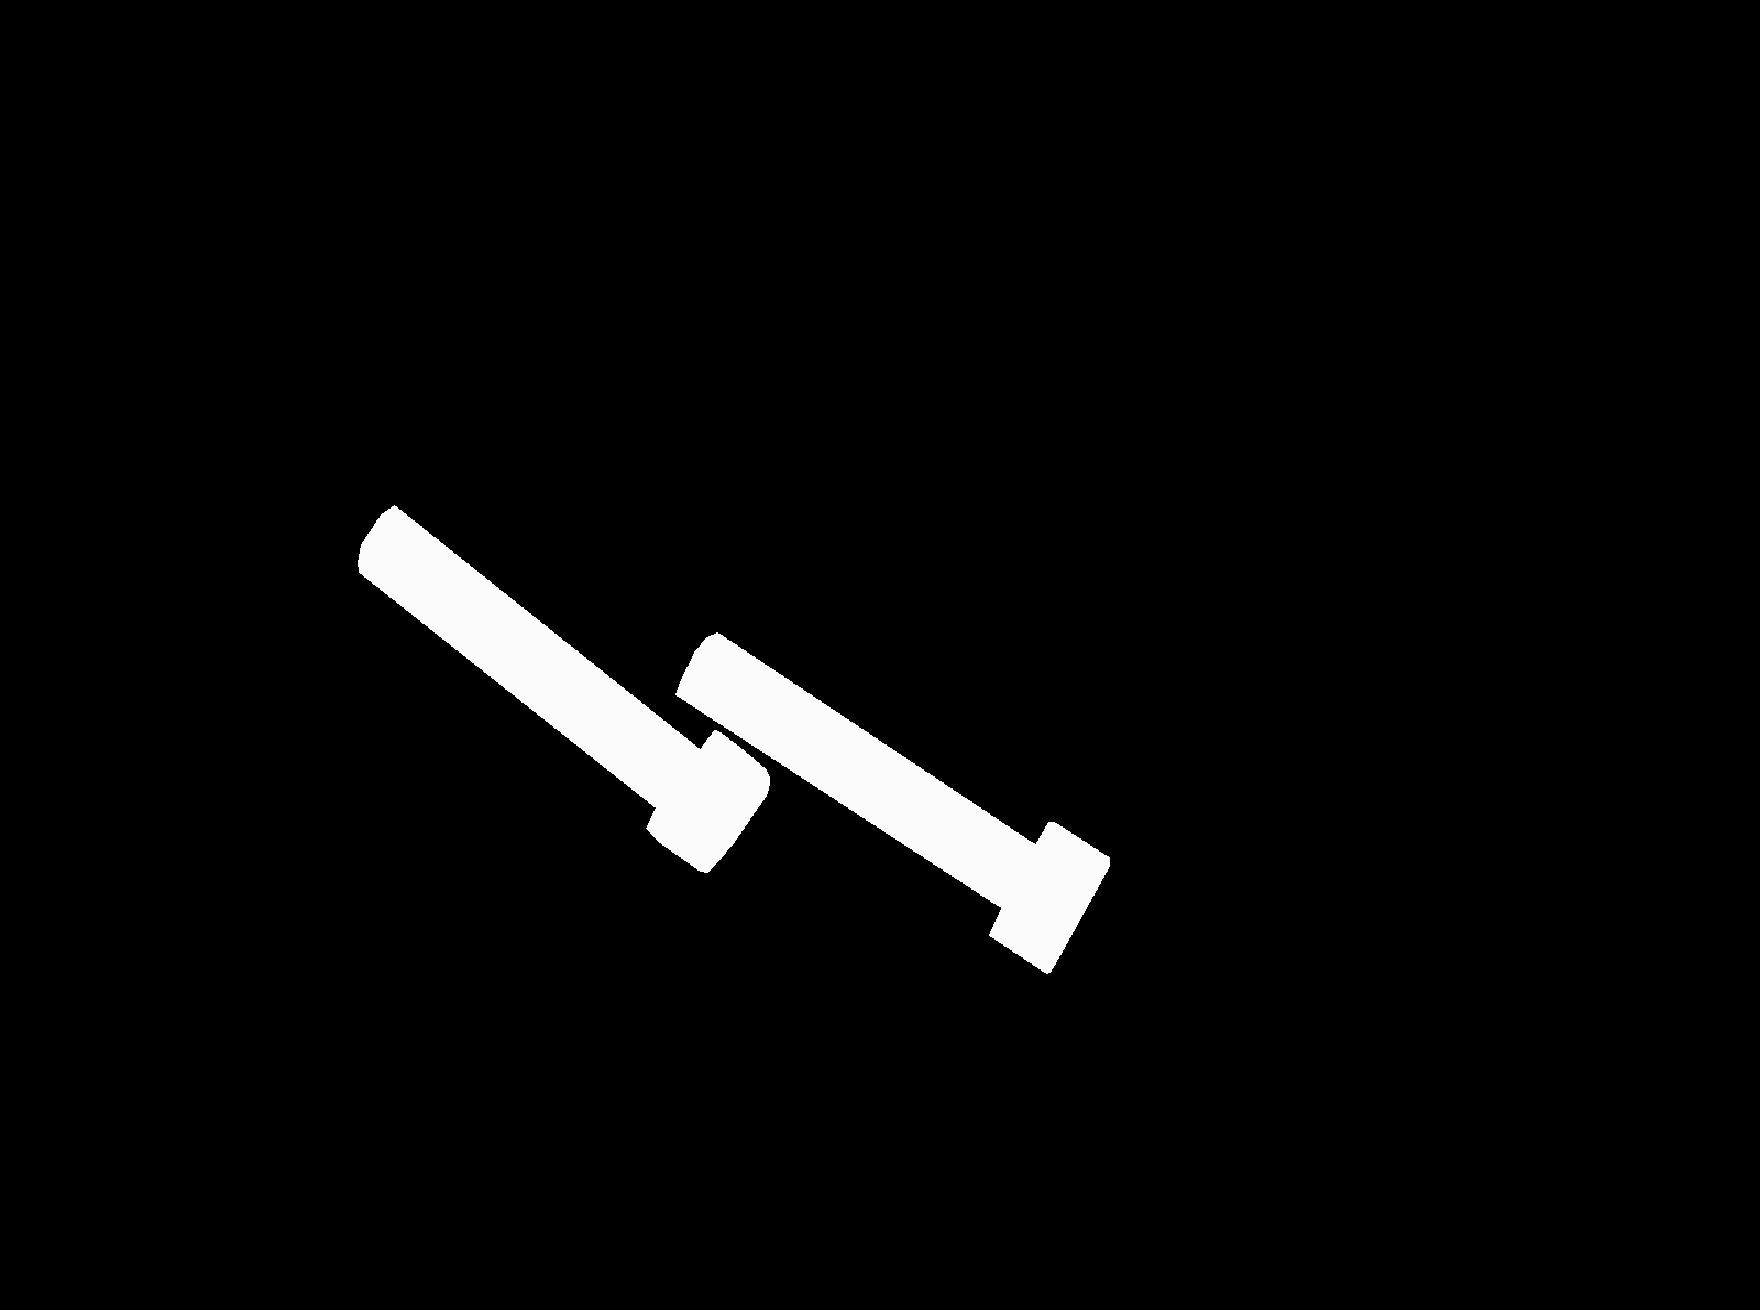
\includegraphics[width=\textwidth]{figures/DRAEMweakness/logical042mask.png}
        \end{minipage}
        \begin{minipage}{0.32\textwidth}
            \centering
            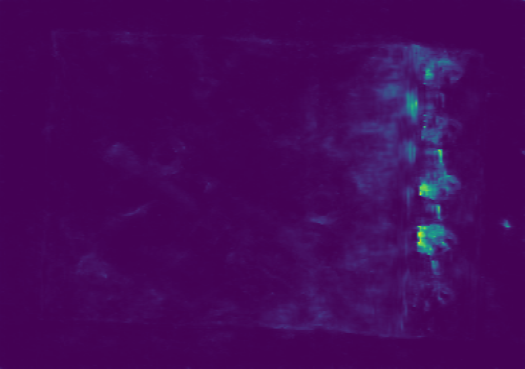
\includegraphics[width=\textwidth]{figures/DRAEMweakness/logical042segment.png}
        \end{minipage}
    \end{subfigure}
    \caption{Example segmentations of DRAEM \cite{Zavrtanik_2021DRAEM}, showcasing its precise segmentation and weakness in localizing missing objects.}
    \label{fig:DRAEMweakness}
\end{figure}

The other classifiers, PatchCore \cite{patchCore2022}, SimpleNet \cite{liu2023simplenet} and Reverse Distillation \cite{revdist2023}, generally showed good performance. Unlike DRAEM, they exhibited 
poorer performance when classifying small anomalies (Fig. \ref{fig:overshoot}). Moreover, the segmentations often slightly overshoot the anomalous regions at various confidence 
degrees. This means that unlike DRAEM \cite{Zavrtanik_2021DRAEM}, which is very strict with segmentation, those approaches tend to segment more pixels than necessary. 
Of course, these pixels do not have the same values, so the performance is still viable after thresholding. 

\begin{figure}[H]
    \captionsetup[subfigure]{justification=centering}
    \centering
    \begin{subfigure}[b]{0.45\textwidth}
        \centering
        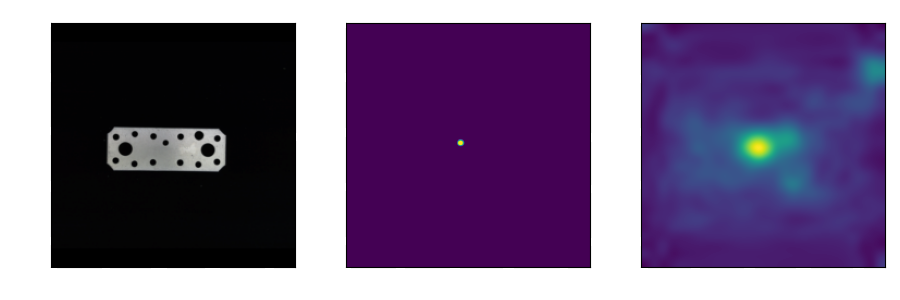
\includegraphics[width=\textwidth]{figures/overshootexamples/flat_connector_test_logical_anomalies_004.png}
        \caption{Example of overshooting image prediction.}

    \end{subfigure}
    \begin{subfigure}[b]{0.45\textwidth}
        \centering
        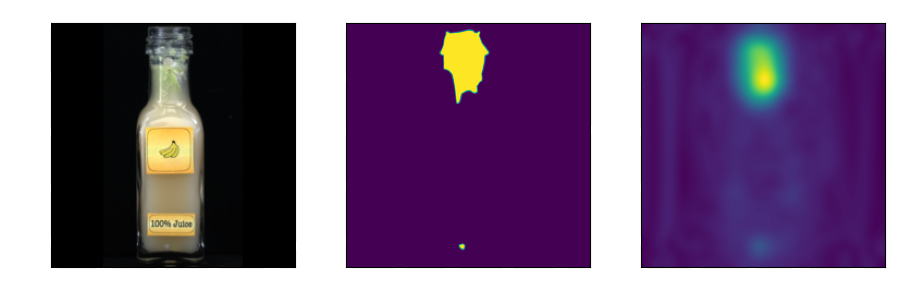
\includegraphics[width=\textwidth]{figures/overshootexamples/juice_bottle_test_structural_anomalies_019.png}
        \caption{Example of smaller anomalous region having significantly less certainty than larger regions.}

    \end{subfigure}
    
    \caption{Exemplary segmentations of representation-based classifiers that showcase less precise segmentaions than reconstruction-based approaches like DRAEM \cite{Zavrtanik_2021DRAEM}.}
    \label{fig:overshoot}
\end{figure}



\section{Flat Connector Experiments}
\label{sec:faltconnectorxperiments}

The experiments on the flat connector class produced high performance from all classifiers participating in the survey. Table \ref{tab:flatconnectorperformance} 
displays an overview of important metrics calculated on this novel class.

\begin{table}[htbp]
    \tiny
    \centering
    \begin{tabularx}{\textwidth}{|X|X|X|X|X|X|X|X|X|X|X|X|X|X|X|X|X|X|}%{|c|p{5cm}|p{5cm}|p{5cm}|}
        \hline
        \textbf{Metric} & \textbf{PatchCore} \cite{patchCore2022} & \textbf{SimpleNet} \cite{liu2023simplenet} & \textbf{CSFlow }\cite{csflow2022} & \textbf{DRAEM} \cite{Zavrtanik_2021DRAEM} & \textbf{Reverse Destillation} \cite{revdist2023} \\
        \hline
        Image AUROC & 0.995 & 1.0 & 0.970 & 0.982 & 0.996 \\
        \hline
        Pixel AUROC & 0.993 & 0.984 & - & 0.995 & 0.992 \\
        \hline
        sPRO & - & - & - & - & - \\
        \hline
    \end{tabularx}
    \caption{Results of this works IAD methods on the novel flat connector dataset class. Evaluates performance in regards to the metrics: image levele AUROC, pixel level AUROC and sPRO}
    \label{tab:flatconnectorperformance}
\end{table}


The localization performances display characteristics similar to those of each classifier during the last experiment. This relates to DRAEMs \cite{Zavrtanik_2021DRAEM} precise segmentation, 
as well as the more fuzzy segmentation of the other classifiers. Below are representative results of the classifier localization performance on the flat connector class (Fig. \ref{fig:FCallapproaches}).



\begin{figure}[htbp]
    \centering
    \captionsetup[subfigure]{justification=centering}
    \begin{subfigure}[b]{\textwidth}
        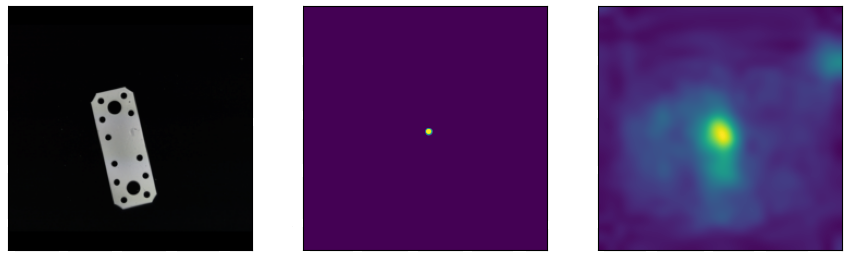
\includegraphics[width=0.45\textwidth]{figures/allapproachesFCimages/patchcore_flat_connector_test_logical_anomalies_023.png}
        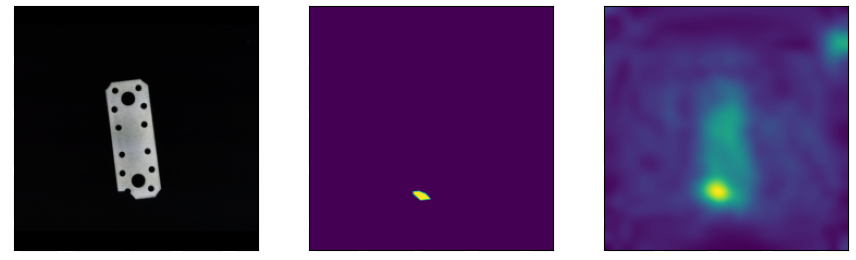
\includegraphics[width=0.45\textwidth]{figures/allapproachesFCimages/patchcore_flat_connector_test_structural_anomalies_014.png}
        \caption{Segmentation results of PatchCore \cite{patchCore2022} on novel dataset class.}
    \end{subfigure}
    \hfill
    \begin{subfigure}[b]{\textwidth}
        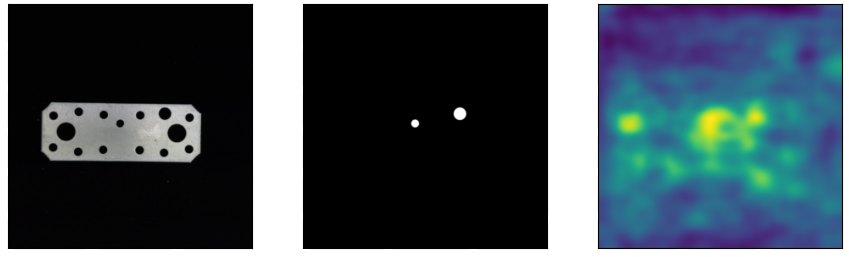
\includegraphics[width=0.45\textwidth]{figures/allapproachesFCimages/simplenet_flat_connector_test_logical_anomalies_004.png}
        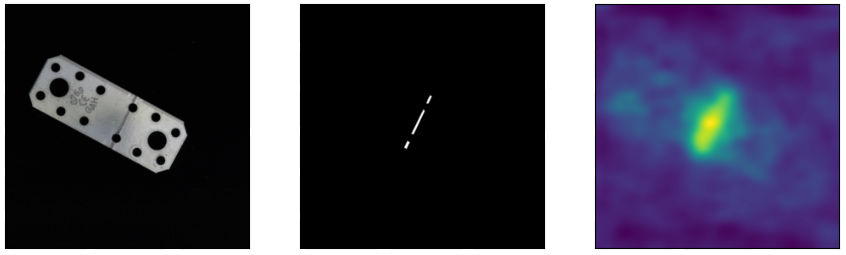
\includegraphics[width=0.45\textwidth]{figures/allapproachesFCimages/simplenet_flat_connector_test_structural_anomalies_016.png}
        \caption{Segmentation results of SimpleNet \cite{liu2023simplenet} on novel dataset class.}
    \end{subfigure}
    \hfill
    \begin{subfigure}[b]{\textwidth}
        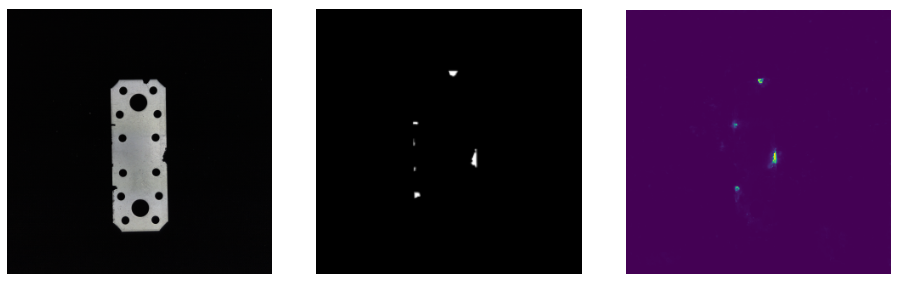
\includegraphics[width=0.45\textwidth]{figures/allapproachesFCimages/DRAEM_structural_26.png}
        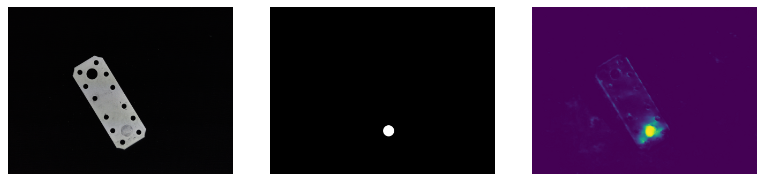
\includegraphics[width=0.45\textwidth]{figures/allapproachesFCimages/DRAEM_logical_image_40.png}
        \caption{Segmentation results of DRAEM \cite{Zavrtanik_2021DRAEM} on novel dataset class.}
    \end{subfigure}
    \begin{subfigure}[b]{\textwidth}
        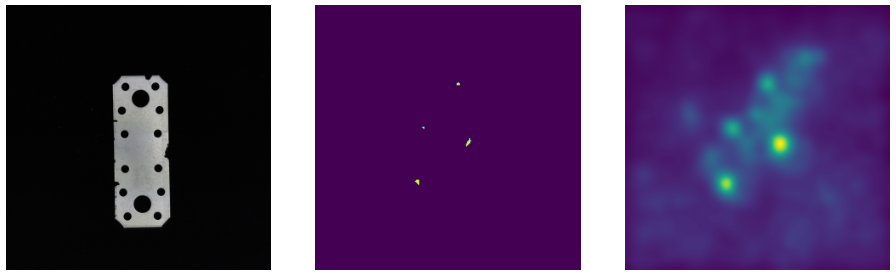
\includegraphics[width=0.45\textwidth]{figures/allapproachesFCimages/RevDist_structural_26.png}
        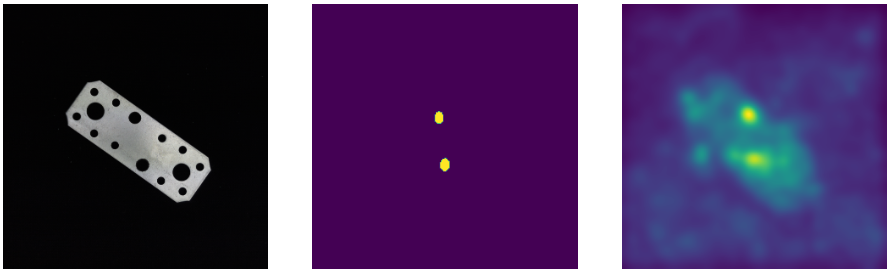
\includegraphics[width=0.45\textwidth]{figures/allapproachesFCimages/RevDist_logical_016.png}
        \caption{Segmentation results of Reverse Distillation \cite{revdist2023} on novel dataset class.}

    \end{subfigure}
    \caption{Localization results of all IAD approaches on the novel flat connector class. One instance image for logial and structural anomalies each per approach.}
    \label{fig:FCallapproaches}
\end{figure}



\section{Ensemble Network}
\label{sec:ensembleresults}

This section reports the results of the ensemble network approach on the class flat connector to facilitate the understanding of visual 
analysis. Furthermore, as the flat connector class seems to be less of a challenge to this work's approaches than other classes, it is convenient to showcase the strengths and 
shortcomings of the ensemble models in a more easy environment. More experiments from other classes of the MVTecAD LOCO \cite{LOCODentsAndScratchesBergmann2022} set are to be found in the appendix. 
Performance reported here is strictly worse in other classes, meaning fewer anomalies could be learned in a more challenging environment. Firstly, the primary ensemble approach results from section \ref{sec:featurelevelensemble} are reported. Afterwards, 
the results of the secondary ensemble approach are presented, supported by metrics and segmentation examples.


\subsection{Independent Transformation Block}
\label{subsec:ITBfail}

The results were generally not meaningful when performing the ensemble training process using the approach by \cite{EnsembleHeller2023}. Looking at the exemplary plot of the segmentation 
results in Fig. \ref{fig:pca_res}, it becomes obvious why no metrics are reported for this experiment. When investigating image level metrics, they were highly inconsistent throughout 
the training process and are regarded as not meaningful and representative.

\begin{figure}[htbp]
    \captionsetup[subfigure]{justification=centering}
    \centering
    \begin{subfigure}[b]{0.3\textwidth}
        \centering
        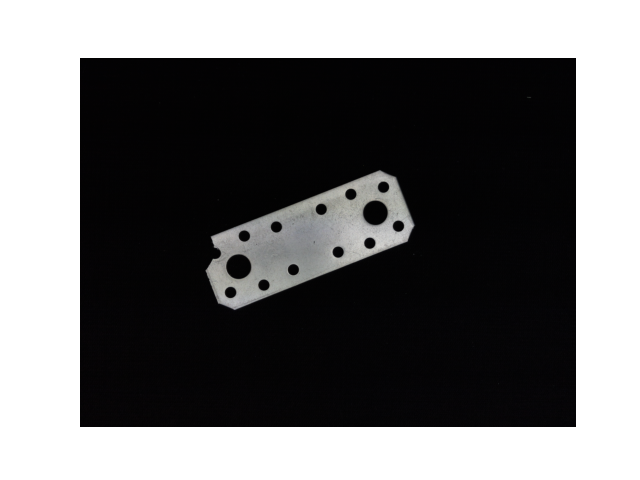
\includegraphics[width=\textwidth]{figures/pca_results/cut_corner.png}
        \caption*{original Image}

    \end{subfigure}
    \begin{subfigure}[b]{0.3\textwidth}
        \centering
        
\includegraphics[width=\textwidth]{figures/pca_results/cut_corner_mask.png}
        \caption*{Mask}

    \end{subfigure}
    \begin{subfigure}[b]{0.3\textwidth}
        \centering
        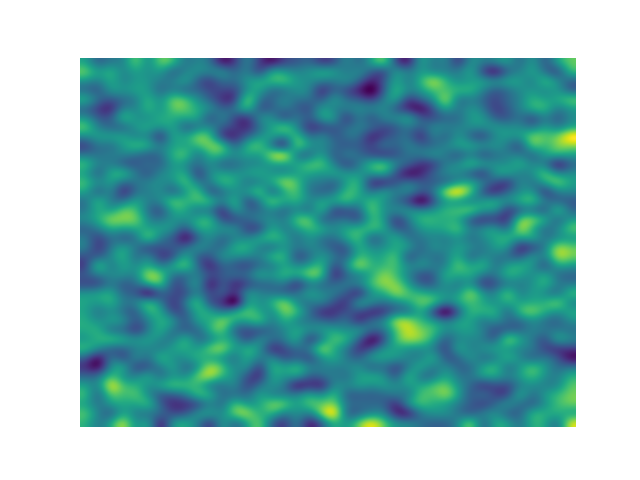
\includegraphics[width=\textwidth]{figures/pca_results/pca_res.png}
        \caption*{Discriminator Predictions}

    \end{subfigure}
    \caption{Results of Independent Transformation Block Ensembles Section \ref{sec:featurelevelensemble}}
    \label{fig:pca_res}
\end{figure}

As visible in Fig. \ref{fig:pca_res}, the segmentation results appeared to be as meaningful as Gaussian noise, strongly suggesting that this method has failed. Subsection 
\ref{subsec:ITBfaildiscussion} will go into possible reasons for the suboptimal experiments results. Concludingly, it is to be said that these results are, besides the failure analysis 
in the conclusion, not relevant and will not be part of further review. Thus, no results from other classes using this method are posted in the appendix.

\subsection{Stacking Ensemble}
\label{subsec:stacking}
This subsection reports the performance of both ensemble experiments with stacking as the ensemble method. 
The experiment is split into two smaller experiments. One investigates the performance of ensembling higher and lower level features in 
single backbones, whereas the other one regards standard backbone ensembling with the ones mentioned in section \ref{sec:ensemblecandidates}. 

\begin{table}[htbp]
    \tiny
    \centering
    \begin{tabularx}{\textwidth}{|X|X|X|X|X|X|X|X|}%{|c|p{5cm}|p{5cm}|p{5cm}|}
        \hline
        \textbf{Method} & \textbf{Breakfast Box} & \textbf{Flat Connector} & \textbf{Juice Bottle} & \textbf{Pushpins} & \textbf{Scew Bag} & \textbf{Splicing Connectors} & \textbf{Average} \\
        \hline
        WR50L23 + R50L23 + R18L23  & 0. & 0.931 & 0. & 0. & 0. & 0. & 0. \\
        \hline
        WR50L12 + WR50L23 & 0.745 & 0.989 & 0.760 & 0.618 & 0.666 & 0.643 & 0.884 \\
        \hline
    \end{tabularx}
    \caption{Ensemble results on MVTecAD LOCO \cite{LOCODentsAndScratchesBergmann2022} by this works introduced ensemble approaches. The leftmost columns represents the ensemble 
             constellation. The abbreviations denote the following: 
             WR50 = wideresnet50, R50 = resnet50, R18 = resnet18. Lxy means an aggreation of layers x and y. Lastly the + sign shows that the listed abbreviations belong to one ensemble.}
    \label{tab:ensembleimageAUROC}
\end{table}







\begin{table}[htbp]
    \tiny
    \centering
    \begin{tabularx}{\textwidth}{|X|X|X|X|X|X|X|X|}%{|c|p{5cm}|p{5cm}|p{5cm}|}
        \hline
        \textbf{Method} & \textbf{Breakfast Box} & \textbf{Flat Connector} & \textbf{Juice Bottle} & \textbf{Pushpins} & \textbf{Scew Bag} & \textbf{Splicing Connectors} & \textbf{Average} \\
        \hline
        WR50L23 + R50L23 + R18L23  & 0.504 & 0.808 & 0.621 & 0.485 & 0.501 & 0.327 & 0.682 \\
        \hline
        WR50L12 + WR50L23 & 0.499 & 0.949 & 0.750 & 0.515 & 0.585 & 0.368 & 0.733 \\
        \hline
    \end{tabularx}
    \caption{Ensemble results on MVTecAD LOCO \cite{LOCODentsAndScratchesBergmann2022} by this works introduced ensemble approaches. The leftmost columns represents the ensemble 
             constellation. The abbreviations denote the following: 
             WR50 = wideresnet50, R50 = resnet50, R18 = resnet18. Lxy means an aggreation of layers x and y. Lastly the + sign shows that the listed abbreviations belong to one ensemble.}
    \label{tab:ensemblepixelAUROC}
\end{table}





\textbf{Hierarchy Levels.} The results of ensembling different hierarchies exhibit a degree of diversity between layer hierarchies. As briefly mentioned in section \ref{sec:ensemblecandidates}, the resnet backbones consist of four 
layers; in other words, they contain four larger sequential blocks. Inference using higher-level feature representations with a backbone of subtype resnet resulted in suboptimal results, segmentation-wise. 
Fig. \ref{fig:faillayersegments} exemplary showcases the segmentation results of training using the wideresnet50 backbone and including a feature aggregation between layers 3 and 4. 



\begin{figure}[htbp]
    \centering
    \begin{subfigure}[b]{0.45\textwidth}
        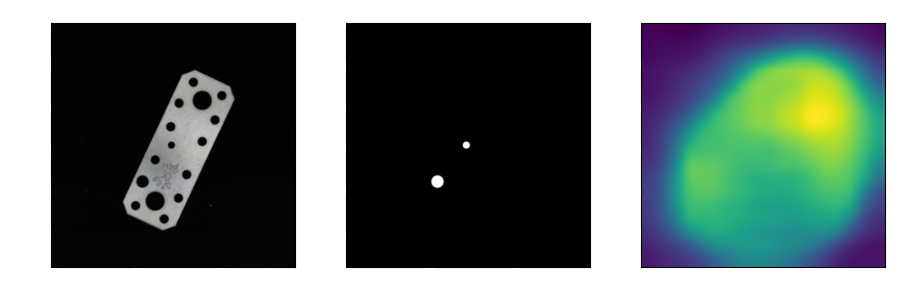
\includegraphics[width=\textwidth]{figures/faillayer34/flat_connector_test_logical_anomalies_001.png}

    \end{subfigure}
    \begin{subfigure}[b]{0.45\textwidth}
        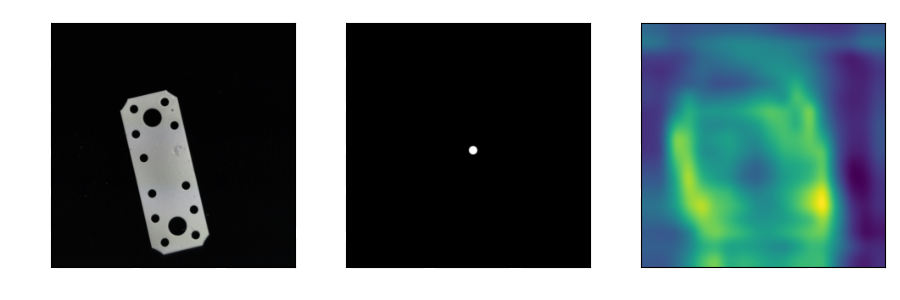
\includegraphics[width=\textwidth]{figures/faillayer34/flat_connector_test_logical_anomalies_023.png}

    \end{subfigure}
    \caption{Resulting segmentations of ensemble network training when utilizing layer 4.}
    \label{fig:faillayersegments}
\end{figure}

The image and pixel AUROC were unstable and poor throughout the training, 
as Fig. \ref{fig:failmetrics} suggests, and therefore were not recorded explicitly for multiple classes, as this was true for all training. The loss visible in Fig. \ref{fig:failmetricsloss} furthermore 
showcases the flawed training process. Due to these findings, the following experiments only consider earlier layers if diverging from the standard layers 
discussed in section \ref{sec:ensemblecandidates}.

\begin{figure}[htbp]
    \centering
    \begin{subfigure}[b]{0.4\textwidth}
        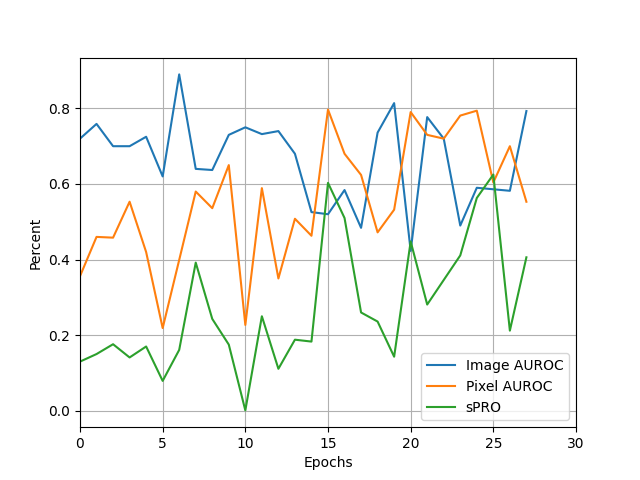
\includegraphics[width=\textwidth]{figures/faillayer34/auprosetc.png}
        \caption{Testing metrics over the course of 30 meta epochs. Usually may contain fluctuations, but not of this amplitude.}
        \label{fig:failmetrics}
    \end{subfigure}
    \begin{subfigure}[b]{0.4\textwidth}
        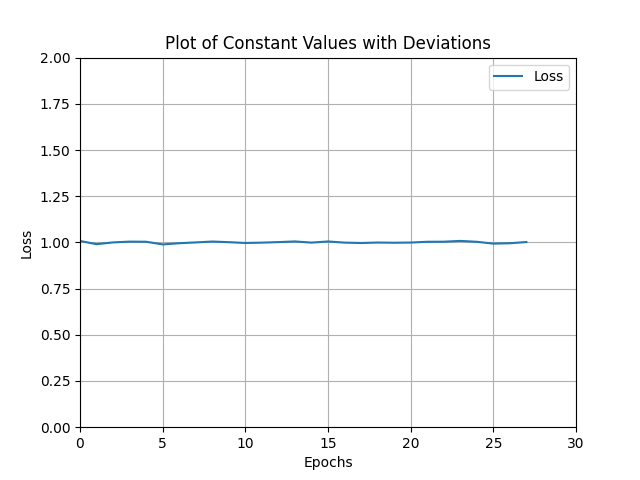
\includegraphics[width=\textwidth]{figures/faillayer34/loss_fail.png}
        \caption{The networks loss during 30 meta epochs. Shows only very little deviations from value 1, not desirable behavior.}
        \label{fig:failloss}
    \end{subfigure}
    \caption{Training metrics and loss of ensemble network training, utilizing layer 4.}
    \label{fig:failmetricsloss}
\end{figure}


Experiments combining lower-layer aggregations yielded different results. Table \ref{tab:ensemblepixelAUROC} summarises the reported pixel metrics on the MVTecAD LOCO \cite{LOCODentsAndScratchesBergmann2022} 
dataset, and Fig. \ref{fig:ensemblehierarchy} showcases exemplary 
segmentation images of the experiments. More data is to be found in the appendix.

\begin{figure}[htbp]
    \captionsetup[subfigure]{justification=centering}
    \centering
    \begin{subfigure}[b]{0.3\textwidth}
        \centering
        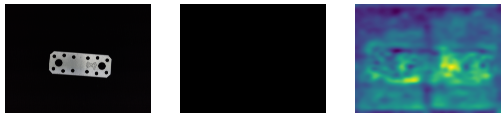
\includegraphics[width=\textwidth]{figures/ensemblehierarchyimages/image_prediction_018.png}
        %\caption*{Logical Anomalies}

    \end{subfigure}
    \begin{subfigure}[b]{0.3\textwidth}
        \centering
        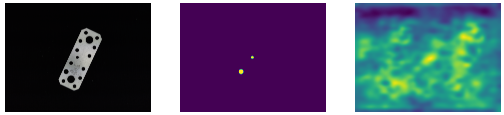
\includegraphics[width=\textwidth]{figures/ensemblehierarchyimages/image_prediction_021.png}


    \end{subfigure}
    \begin{subfigure}[b]{0.3\textwidth}
        \centering
        \includegraphics[width=\textwidth]{figures/ensemblehierarchyimages/image_prediction_047.png}


    \end{subfigure}
    \begin{subfigure}[b]{0.3\textwidth}
        \centering
        \includegraphics[width=\textwidth]{figures/ensemblehierarchyimages/image_prediction_064.png}
        %\caption*{Structural Anomalies}

    \end{subfigure}
    \begin{subfigure}[b]{0.3\textwidth}
        \centering
        \includegraphics[width=\textwidth]{figures/ensemblehierarchyimages/image_prediction_071.png}


    \end{subfigure}
    \begin{subfigure}[b]{0.3\textwidth}
        \centering
        \includegraphics[width=\textwidth]{figures/ensemblehierarchyimages/image_prediction_089.png}


    \end{subfigure}
    \caption{Representative segmentation results from our stacking ensemble with multiple Wideresnet50 backbones at the various hierarchy level. The predictions are done on the novel flat 
             connector class.}
    \label{fig:ensemblehierarchy}
\end{figure}

Here, it is to be seen that, at least for this class, the anomalies are segmented. The localization performance seems to be worse than the standard SimpleNet \cite{liu2023simplenet} 
performance, judging from segmentation images (Fig. \ref{fig:ensemblehierarchy}) and metrics (Tab. \ref{tab:ensembleimageAUROC}, Tab. \ref{tab:ensemblepixelAUROC}). While the anomalous regions often still get detected, there is a lot more uncertainty regarding 
the pixel scores than from comparable IAD approaches, leading to less robust results. In other experiments in the appendix, this performance is significantly worse on 
other classes like the splicing connectors.



\textbf{Backbone Ensemble.} The performance of this approach is visible in table \ref{tab:ensembleimageAUROC}. The performance is visibly worse than the performance 
reported by the standard simple approach. However, the results suggest some learning process for the flat connector class, unlike the experiment conducted in section \ref{subsec:ITBfail}. 
Moreover, the loss, presented in Fig. \ref{fig:ensembleloss}, suggests a conceptually adequate learning. The performance could not be increased by a higher 
epoch count, as seen by the loss progression in the other subfigure.

\begin{figure}[ht]
    \captionsetup[subfigure]{justification=centering}
    \centering
    \begin{subfigure}[b]{0.45\textwidth}
        \centering
        \includegraphics[width=\textwidth]{figures/ensemble_losses/normal_ensemble_loss.png}

    \end{subfigure}
    %\hfill
    \begin{subfigure}[b]{0.45\textwidth}
        \centering
        \includegraphics[width=\textwidth]{figures/ensemble_losses/long_ensemble_loss.png}

    \end{subfigure}
    

    \caption{Loss of ensemble network using the three standard backbones next to loss of the same network with increased meta epochs and increased discriminator epochs. Not significant difference 
             in loss can be seen after training to new convergence.}
    \label{fig:ensembleloss}
\end{figure}

Moreover Fig. \ref{fig:ensembleFCimages} showcases exemplary segmentation results on the flat connector class. As 
seen, the ensemble outputs consist of much more uncertainty, as the values are closer together and visually harder to distinguish. This uncertainty 
was higher for logical anomalies than for structural ones. Still, 
using thresholding, the approach is viable, as anomalous regions are often discernible. Fig. \ref{fig:ensembleFCimages} also showcases examples of failed segmentation 
attempts. 

\begin{figure}[htbp]
    \captionsetup[subfigure]{justification=centering}
    \centering
    \begin{subfigure}[b]{0.3\textwidth}
        \centering
        \includegraphics[width=\textwidth]{figures/ensembleimagesFC/image_prediction_100.png}
        %\caption*{Logical Anomalies}

    \end{subfigure}
    \begin{subfigure}[b]{0.3\textwidth}
        \centering
        \includegraphics[width=\textwidth]{figures/ensembleimagesFC/image_prediction_036.png}


    \end{subfigure}
    \begin{subfigure}[b]{0.3\textwidth}
        \centering
        \includegraphics[width=\textwidth]{figures/ensembleimagesFC/image_prediction_052.png}


    \end{subfigure}
    \begin{subfigure}[b]{0.3\textwidth}
        \centering
        \includegraphics[width=\textwidth]{figures/ensembleimagesFC/image_prediction_061.png}
        %\caption*{Structural Anomalies}

    \end{subfigure}
    \begin{subfigure}[b]{0.3\textwidth}
        \centering
        \includegraphics[width=\textwidth]{figures/ensembleimagesFC/image_prediction_073.png}


    \end{subfigure}
    \begin{subfigure}[b]{0.3\textwidth}
        \centering
        \includegraphics[width=\textwidth]{figures/ensembleimagesFC/image_prediction_085.png}


    \end{subfigure}
    \caption{Representative segmentation results from our stacking ensemble with different residual network backbones at the same hierarchy level. The predictions are done on the novel flat 
             connector class.}
    \label{fig:ensembleFCimages}
\end{figure}

As a comparison, Fig. \ref{fig:singlebackboneexamples} displays example segmentations from the individual backbones. Here, there is less uncertainty or 
noise than in the ensembled approach. This makes for worse and less robust ensemble performance, especially regarding segmentation. 
The implications and reasons for this are taken up in the next chapter.


\begin{figure}[htbp]
    \centering
    \begin{subfigure}[b]{0.4\textwidth}
        \includegraphics[width=\textwidth]{figures/backboneexamples/flat_connector_test_logical_anomalies_033.png}

    \end{subfigure}
    \begin{subfigure}[b]{0.4\textwidth}
        \includegraphics[width=\textwidth]{figures/backboneexamples/flat_connector_test_structural_anomalies_001.png}

    \end{subfigure}
    \caption{Instance segmentations from backbones Wideresnet50 \cite{wideresnet} and Resnet50 \cite{He_2016resnet} on the novel flat connector class.}
    \label{fig:faillayersegments}
\end{figure}




